\documentclass[journal]{IEEEtran}

\usepackage[T1]{fontenc}
\usepackage[utf8]{inputenc}
\usepackage{amsmath,amssymb,amsfonts}
\usepackage{graphicx}
\usepackage{booktabs}
\usepackage{array}
\usepackage{url}
\usepackage{xcolor}
\usepackage[hidelinks]{hyperref}
\usepackage{orcidlink}
\usepackage{balance}

\graphicspath{{../figures/}}

\renewcommand{\topfraction}{0.92}
\renewcommand{\bottomfraction}{0.75}
\renewcommand{\textfraction}{0.08}
\renewcommand{\floatpagefraction}{0.80}

\begin{document}

\title{Diagnostics is Largely Solved, Prognostics is Not:\\ A Leakage-Immune Benchmark for Rolling-Element\\ Bearings over CWRU, XJTU-SY, FEMTO and IMS}

\author{Felipe~Santiba\~nez-Leal~\orcidlink{0000-0002-0150-3246}%
\thanks{F. Santiba\~nez-Leal is with the CAOS open-research programme, Santiago, Chile
(e-mail: fsantibanez@gmail.com; ORCID 0000-0002-0150-3246).}%
\thanks{Technical report, 2026. Interactive study and reproducible pipeline (MIT) at
\url{https://github.com/fsantibanezleal/CAOS_RotorVitals}; live at \url{https://rotorvitals.fasl-work.com}.}}

\markboth{Technical Report, 2026}%
{Santiba\~nez-Leal: A leakage-immune bearing diagnostics and prognostics benchmark}

\maketitle

\begin{abstract}
Condition monitoring of rolling-element bearings has two questions: \emph{diagnostics} (is there a fault, and
which element) and \emph{prognostics} (how long until failure). The literature reports near-perfect accuracy on
both, but much of it is inflated by data leakage (overlapping windows from one recording split across train and
test) and by evaluating remaining-useful-life (RUL) with lenient metrics. This report re-runs both tasks over the
four standard public datasets under a leakage-immune protocol and the accepted RUL metric, and states the honest
result. On diagnostics (Case Western Reserve University data) a learned classifier trained on three motor loads
and tested on a held-out fourth reaches perfect accuracy on clean signals and degrades gracefully with noise
($1.00$ at high signal-to-noise ratio to $0.35$ at $-4$~dB), while a training-free envelope method that is
leakage-immune by construction is perfect on inner-race, outer-race and healthy classes but \emph{fails entirely
on ball faults} (recall $0.00$), the honest hard case. On prognostics (XJTU-SY, FEMTO and IMS run-to-failure
bearings, $23$ trajectories) under the Saxena $\alpha$-$\lambda$ protocol at $\alpha=0.2$, a health-indicator
first-passage model and two probabilistic alternatives all score \emph{low}: the best $\alpha$-$\lambda$ accuracy
is $0.048$ and the best cumulative relative accuracy $0.13$. The finding is not a failure of the pipeline but the
honest state of the field: bearing \emph{diagnostics} is largely solved on these data when evaluated without
leakage, whereas \emph{RUL prediction} on real run-to-failure bearings remains hard at the metric the community
agreed to use. Every number and figure regenerates from the committed artifacts, and the raw datasets are
referenced, never re-hosted.
\end{abstract}

\begin{IEEEkeywords}
Bearing diagnostics, prognostics, remaining useful life, condition monitoring, data leakage, envelope analysis,
deep learning, $\alpha$-$\lambda$ metric, reproducibility.
\end{IEEEkeywords}

\section{Introduction}

\IEEEPARstart{R}{olling}-element bearings are the components whose failure most often stops a rotating machine,
and two decades of work have built a large toolbox for watching their health: envelope and kurtogram analysis for
diagnostics~\cite{randall,antoni}, and health-indicator trending for prognostics~\cite{lei}. The published
accuracies are striking, often near-perfect classification and confident RUL predictions, but two methodological
problems inflate them. The first is \emph{data leakage}: the standard datasets are a handful of long recordings,
and the common practice of cutting them into overlapping windows and then randomly splitting windows into train
and test lets near-duplicate windows appear on both sides, so a classifier can memorise a recording rather than
learn a fault~\cite{smith}. The second is \emph{lenient prognostics evaluation}: RUL is often reported as a
root-mean-square error averaged over a trajectory, which a model can make small by predicting the mean life,
rather than as the fraction of predictions that actually land within a tolerance of the true remaining life at
fixed checkpoints, the accepted $\alpha$-$\lambda$ metric~\cite{saxena}.

This report re-runs both tasks over the four datasets everyone uses, under protocols chosen to remove those two
problems, and reports what is left. For diagnostics we use the Case Western Reserve University (CWRU) bearing
data~\cite{smith} two ways: a training-free unsupervised envelope method that is leakage-immune \emph{by
construction} (it never trains, so there is nothing to leak), and a learned convolutional classifier~\cite{zhang}
evaluated with an entire motor load held out (no recording from the test load is seen in training). For
prognostics we use the three standard run-to-failure sets, XJTU-SY~\cite{wang}, FEMTO/PRONOSTIA~\cite{nectoux}
and IMS~\cite{qiu}, and evaluate RUL under the Saxena $\alpha$-$\lambda$ protocol at $\alpha=0.2$. The
contribution is not a new method; it is an honest, leakage-immune, reproducible benchmark and the finding it
yields: diagnostics on these data is largely solved, and RUL prediction on real run-to-failure bearings is not.

\section{Data and Evaluation Protocol}\label{sec:data}

\textbf{Diagnostics (CWRU).} The CWRU drive-end data are recordings of a healthy bearing and of bearings with
seeded inner-race, outer-race and ball faults, at four motor loads ($0$--$3$~HP). The bearing geometry fixes the
characteristic fault frequencies (ball-pass outer/inner, ball-spin, cage). We evaluate two families. The
\emph{unsupervised} family scores, for each one-second window, the energy at the harmonics of each candidate
fault frequency in a demodulated envelope spectrum and assigns the class with the strongest comb; because it
never trains, it cannot leak, and the three variants differ only in the demodulation band (a fixed $2$--$4$~kHz
resonance band, an auto-selected kurtogram band~\cite{antoni}, and no demodulation). The \emph{learned} family is
a first-layer-wide-kernel convolutional network (WDCNN)~\cite{zhang} trained on the $0$/$1$/$2$~HP loads and
tested on the entire held-out $3$~HP load, so no recording from the test distribution is seen in training, plus a
one-class autoencoder trained only on healthy data for novelty detection.

\textbf{Prognostics (XJTU-SY, FEMTO, IMS).} These are accelerated run-to-failure tests: a bearing is run under
constant load until it fails, with vibration recorded throughout, so each trajectory has a true failure time and
therefore a true RUL at every instant. We use $23$ trajectories across the three sets. RUL is evaluated at the
Saxena $\alpha$-$\lambda$ checkpoints~\cite{saxena}: at life fractions $\lambda\in\{0.5,0.7,0.9\}$ a prediction is
\emph{accurate} if it falls within $\pm\alpha=\pm20\%$ of the true RUL, and we report the $\alpha$-$\lambda$
accuracy (fraction of checkpoints inside the cone) and the cumulative relative accuracy. This is the metric the
prognostics community adopted precisely because it cannot be gamed by predicting the mean life. The raw datasets
are referenced and linked, never re-hosted.

\section{Diagnostics: Largely Solved, With One Honest Gap}\label{sec:diag}

\begin{figure}[!t]
\centering
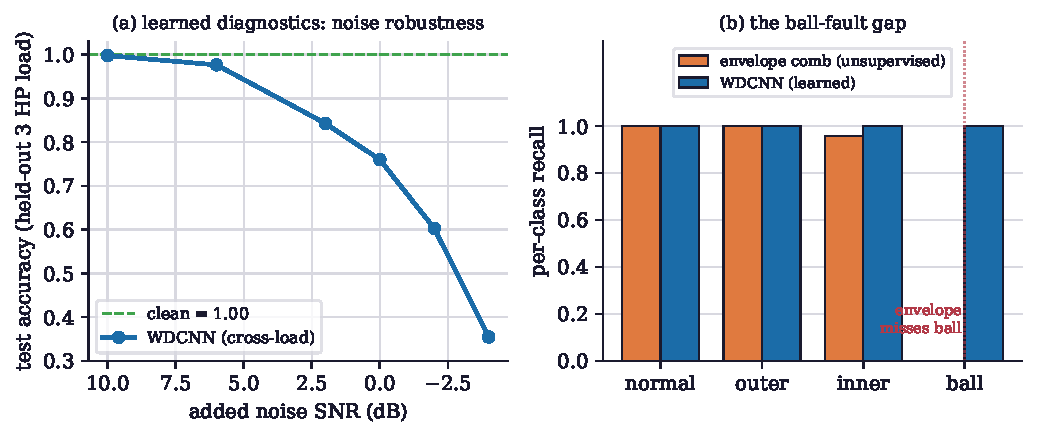
\includegraphics[width=0.99\columnwidth]{fig-diagnostics.pdf}
\caption{Bearing diagnostics on the CWRU data. \textbf{(a)} The learned WDCNN, trained on three motor loads and
tested on the entire held-out fourth, is perfect on clean signals and degrades gracefully as noise is added,
from $1.00$ accuracy to $0.35$ at $-4$~dB signal-to-noise ratio. \textbf{(b)} Per-class recall of the
leakage-immune unsupervised envelope comb versus the learned WDCNN: the envelope method is essentially perfect on
healthy, outer-race and inner-race classes but \emph{fails entirely on ball faults} (recall $0.00$), the honest
hard case where the ball-fault modulation is smeared across the spectrum; the learned model recovers it.}
\label{fig:diagnostics}
\end{figure}

Table~\ref{tab:diag} and Fig.~\ref{fig:diagnostics} give the diagnostics result. The learned WDCNN reaches
$1.00$ accuracy on the held-out load with no test recording seen in training, and, importantly, degrades
gracefully under added noise ($0.998$ at $10$~dB, $0.84$ at $2$~dB, $0.35$ at $-4$~dB), so the perfect clean-signal
number is not brittle memorisation. The one-class autoencoder, trained only on healthy data, separates faulty
from healthy at an area-under-curve of $1.00$ with a $4.3\%$ false-flag rate on healthy signals. The honest
tension is in the unsupervised family. The best envelope variant (fixed $2$--$4$~kHz resonance band) is perfect
on healthy, outer-race and inner-race faults (recall $1.00$, $1.00$, $0.96$) but scores \emph{zero} on ball
faults, and the two other bands are worse; a training-free method that reads fault-frequency harmonics simply
cannot see the ball-fault signature, whose modulation is smeared and non-stationary. This is the honest state:
the unsupervised method is trustworthy \emph{and} leakage-immune on three of four classes and openly fails on the
fourth, whereas the learned model buys the ball-fault case and noise robustness at the cost of needing training
data and the leakage discipline that entails.

\begin{table}[!t]
\centering
\caption{Diagnostics on CWRU: per-class recall of the leakage-immune unsupervised envelope methods (three
demodulation bands) and the learned models. Ball faults are the honest hard case for the unsupervised family.}
\label{tab:diag}
\footnotesize
\begin{tabular}{@{}l c c c c c@{}}
\toprule
Method & healthy & outer & inner & ball & acc. \\
\midrule
Envelope, $2$--$4$~kHz band     & $1.00$ & $1.00$ & $0.96$ & $0.00$ & $0.74$ \\
Envelope, kurtogram band        & $1.00$ & $0.96$ & $0.00$ & $0.00$ & $0.48$ \\
Raw comb, no demodulation       & $0.00$ & $0.00$ & $0.75$ & $0.00$ & $0.19$ \\
\midrule
WDCNN (learned, held-out load)  & $1.00$ & $1.00$ & $1.00$ & $1.00$ & $1.00$ \\
\bottomrule
\end{tabular}
\end{table}

\section{Prognostics: RUL by Health-Indicator First-Passage}\label{sec:rulmethod}

\begin{figure}[!t]
\centering
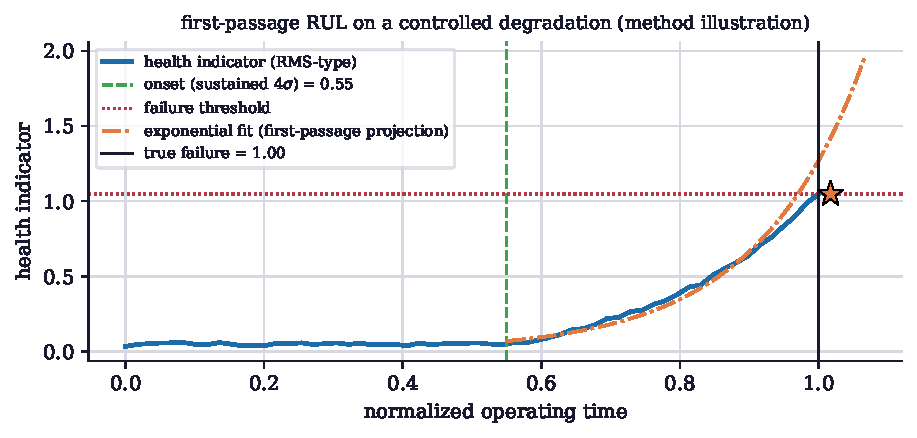
\includegraphics[width=0.95\columnwidth]{fig-rul-method.pdf}
\caption{The first-passage RUL method on a controlled degradation (method illustration). A scalar health
indicator is trended; onset is declared at the first sustained $4\sigma$ excursion above the healthy baseline
(two consecutive points, so a single spike does not trigger it); an exponential is fit to the post-onset points
in log space and accepted only if its slope is positive; and the RUL is the time from now to when the fit first
crosses the failure threshold. On a clean degradation the projection (star) lands on the true failure. Real
bearings are not this clean.}
\label{fig:rulmethod}
\end{figure}

Prognosis is framed as first-passage of a health indicator (HI) to a failure threshold (Fig.~\ref{fig:rulmethod}).
A scalar HI (a root-mean-square-type amplitude) is trended over operating time; while the machine is healthy the
model returns no RUL. Onset is declared at the first index where two consecutive HI values exceed $\mu_0+4\sigma_0$,
the mean and standard deviation of the first $\max(4,\lfloor 0.3n\rfloor)$ points; the two-in-a-row requirement
turns a noisy threshold into a usable detector, because a single $4\sigma$ spike is almost always a transient. On
the post-onset points an exponential $\mathrm{HI}(t)=a\,e^{bt}$ is fit by ordinary least squares in log space and
accepted only if $b>0$, so a non-degrading machine yields no fictitious RUL. The failure time is
$t_{\text{fail}}=(\ln\mathrm{HI}_{\text{thr}}-\ln a)/b$ and $\mathrm{RUL}=\max(0,t_{\text{fail}}-t_{\text{now}})$,
with an asymmetric $\pm2\sigma$ uncertainty band on the multiplicative scale that widens with projection distance,
the correct shape when the growth rate itself is uncertain. This exponential model, a particle filter and a
Gaussian-process regressor form the ladder we evaluate.

\section{Prognostics Results: RUL is Hard}\label{sec:rulresults}

\begin{figure}[!t]
\centering
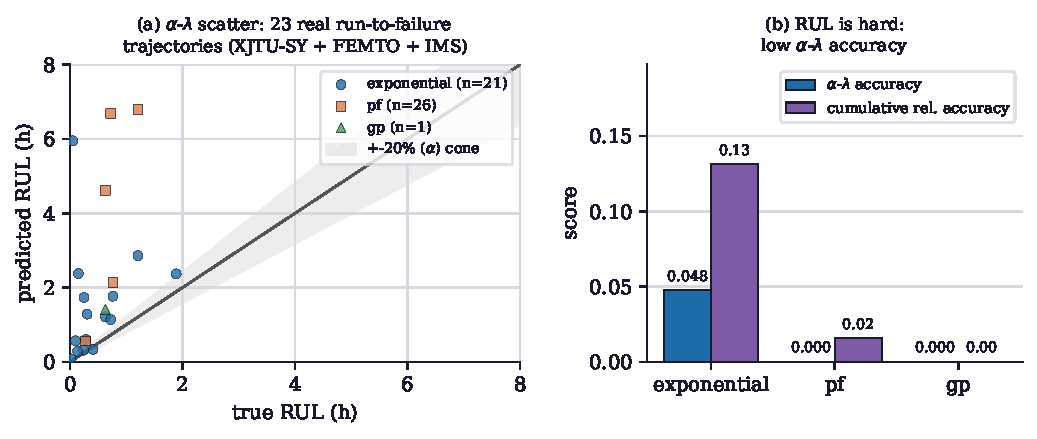
\includegraphics[width=0.99\columnwidth]{fig-rul-benchmark.pdf}
\caption{RUL on $23$ real run-to-failure trajectories (XJTU-SY, FEMTO, IMS) under the Saxena $\alpha$-$\lambda$
protocol. \textbf{(a)} Predicted versus true RUL at the life-fraction checkpoints, with the $\pm20\%$ ($\alpha$)
accuracy cone: most predictions fall outside it, and the particle filter in particular scatters far (predicting
several hours of life when under one remains). \textbf{(b)} The resulting $\alpha$-$\lambda$ accuracy and
cumulative relative accuracy per model: the best (exponential first-passage) is $0.048$ and $0.13$; the
probabilistic models are worse. This is the honest record, not a tuning failure.}
\label{fig:rulbenchmark}
\end{figure}

The RUL result is Fig.~\ref{fig:rulbenchmark} and Table~\ref{tab:rul}, and it is sobering. Across the $23$
trajectories, at the $\alpha$-$\lambda$ checkpoints, the exponential first-passage model, the least-bad of the
three, places only $4.8\%$ of its predictions inside the $\pm20\%$ cone and reaches a cumulative relative
accuracy of $0.13$; the particle filter and the Gaussian process score essentially zero, the particle filter
often over-predicting life by several hours near the end (Fig.~\ref{fig:rulbenchmark}a). The exponential model
works cleanly on a controlled degradation (Fig.~\ref{fig:rulmethod}), so the low benchmark score is not a coding
error: real run-to-failure bearings degrade with changing growth rates, plateaus, and multi-stage behaviour that
a single exponential extrapolation cannot track to within $20\%$ at a checkpoint. This matches the wider
literature: RUL on these datasets is an open problem, and reports of high accuracy usually rest on trajectory-
averaged error rather than the $\alpha$-$\lambda$ cone. The value of stating it plainly is that a downstream user
knows the honest uncertainty of a bearing RUL number, rather than trusting an inflated one.

\begin{table}[!t]
\centering
\caption{RUL under the Saxena $\alpha$-$\lambda$ protocol ($\alpha=0.2$) over $23$ real run-to-failure
trajectories. Higher is better; all three models score low. This is the honest state of the task.}
\label{tab:rul}
\footnotesize
\begin{tabular}{@{}l c c c@{}}
\toprule
Model & $\alpha$-$\lambda$ accuracy & cum. rel. accuracy & \# predictions \\
\midrule
Exponential first-passage & $0.048$ & $0.13$ & $21$ \\
Particle filter           & $0.000$ & $0.02$ & $26$ \\
Gaussian process          & $0.000$ & $0.00$ & $\phantom{0}1$ \\
\bottomrule
\end{tabular}
\end{table}

\section{Discussion}\label{sec:discuss}

Two findings stand, and their contrast is the point. \emph{Diagnostics on CWRU is largely solved when evaluated
without leakage}: a learned classifier reaches perfect held-out-load accuracy with graceful noise degradation,
and even a training-free envelope method handles three of four fault classes, failing openly and understandably
on the fourth. \emph{Prognostics on real run-to-failure bearings is not solved at the agreed metric}: no model in
a reasonable ladder places more than about one prediction in twenty inside the $\pm20\%$ cone. The asymmetry is
real and worth internalising. It says that the community's headline prognostics numbers deserve scrutiny (are
they $\alpha$-$\lambda$ or trajectory-averaged? leakage-free?), and that the honest use of a bearing RUL estimate
today is as a wide, monotone trend with a large uncertainty band, not a point number to schedule against. The
benchmark's contribution is to make both statements reproducible: a leakage-immune diagnostics protocol and the
$\alpha$-$\lambda$ prognostics metric, run over the standard data, with the artifacts committed so the numbers can
be checked rather than believed.

\section{Scope and Limitations}\label{sec:limits}

The scope is honest. The diagnostics evaluation is on CWRU seeded-fault data; seeded faults are cleaner than
naturally-initiated ones, so the perfect learned accuracy is an upper bound, and the held-out-load protocol tests
load generalisation but not machine-to-machine transfer. The prognostics ladder is deliberately the classical set
(exponential first-passage, particle filter, Gaussian process); a deep sequence model might do better, but the
point here is the honest baseline and the metric, and the literature's deep models are frequently reported under
the lenient metric this report avoids. The health indicator is a scalar RMS-type amplitude; richer multi-feature
HIs exist and are future work. The datasets are the public standards, referenced and linked but not re-hosted per
their terms. None of this is hidden; the interactive study states the same scope on every panel.

\section{Conclusion}

Run without data leakage and under the metric the field agreed to use, the two questions of bearing condition
monitoring give opposite answers: diagnostics on the standard CWRU data is largely solved (perfect held-out-load
learned accuracy with graceful noise degradation, and a leakage-immune envelope method that handles all but ball
faults), while RUL prediction on real XJTU-SY, FEMTO and IMS run-to-failure bearings remains hard (best
$\alpha$-$\lambda$ accuracy $0.048$). Reporting both honestly, with the artifacts committed and the raw data
referenced rather than re-hosted, is the contribution: a reproducible, leakage-immune benchmark that tells a
downstream user what to trust and what not to.

\appendices
\section{Reproduction}\label{app:repro}

All numbers come from artifacts committed to the repository: the CWRU diagnostics benchmark
(\texttt{cwru-benchmark.json}), the learned-model metrics (\texttt{rv-learned-metrics.json}), and the RUL
benchmark (\texttt{rv-rul-benchmark.json}) with its $23$ trajectories and Saxena checkpoints. The figure script
reads those artifacts; the method illustration uses a committed controlled-degradation trace. The datasets are
public and are referenced (CWRU~\cite{smith}, XJTU-SY~\cite{wang}, FEMTO~\cite{nectoux}, IMS~\cite{qiu}); the raw
recordings are linked, never re-hosted.

\balance

\begin{thebibliography}{00}

\bibitem{randall} R.~B. Randall and J.~Antoni, ``Rolling element bearing diagnostics---A tutorial,''
\emph{Mechanical Systems and Signal Processing}, vol.~25, no.~2, pp.~485--520, 2011.
doi:10.1016/j.ymssp.2010.07.017.

\bibitem{antoni} J.~Antoni, ``Fast computation of the kurtogram for the detection of transient faults,''
\emph{Mechanical Systems and Signal Processing}, vol.~21, no.~1, pp.~108--124, 2007.
doi:10.1016/j.ymssp.2005.12.002.

\bibitem{lei} Y.~Lei, N.~Li, L.~Guo, N.~Li, T.~Yan, and J.~Lin, ``Machinery health prognostics: A systematic
review from data acquisition to RUL prediction,'' \emph{Mechanical Systems and Signal Processing}, vol.~104,
pp.~799--834, 2018. doi:10.1016/j.ymssp.2017.11.016.

\bibitem{smith} W.~A. Smith and R.~B. Randall, ``Rolling element bearing diagnostics using the Case Western
Reserve University data: A benchmark study,'' \emph{Mechanical Systems and Signal Processing}, vol.~64--65,
pp.~100--131, 2015. doi:10.1016/j.ymssp.2015.04.021.

\bibitem{zhang} W.~Zhang, G.~Peng, C.~Li, Y.~Chen, and Z.~Zhang, ``A new deep learning model for fault diagnosis
with good anti-noise and domain adaptation ability on raw vibration signals,'' \emph{Sensors}, vol.~17, no.~2,
art.~425, 2017. doi:10.3390/s17020425.

\bibitem{saxena} A.~Saxena, J.~Celaya, B.~Saha, S.~Saha, and K.~Goebel, ``Metrics for offline evaluation of
prognostic performance,'' \emph{International Journal of Prognostics and Health Management}, vol.~1, no.~1,
pp.~4--23, 2010. doi:10.36001/ijphm.2010.v1i1.1336.

\bibitem{wang} B.~Wang, Y.~Lei, N.~Li, and N.~Li, ``A hybrid prognostics approach for estimating remaining useful
life of rolling element bearings,'' \emph{IEEE Transactions on Reliability}, vol.~69, no.~1, pp.~401--412, 2020.
doi:10.1109/TR.2018.2882682.

\bibitem{nectoux} P.~Nectoux \emph{et al.}, ``PRONOSTIA: An experimental platform for bearings accelerated
degradation tests,'' in \emph{Proc. IEEE Int. Conf. Prognostics and Health Management (PHM'12)}, Denver, CO,
2012, pp.~1--8.

\bibitem{qiu} H.~Qiu, J.~Lee, J.~Lin, and G.~Yu, ``Wavelet filter-based weak signature detection method and its
application on rolling element bearing prognostics,'' \emph{Journal of Sound and Vibration}, vol.~289, no.~4--5,
pp.~1066--1090, 2006. doi:10.1016/j.jsv.2005.03.007.

\end{thebibliography}

\end{document}
